\subsection{Study area: Portugal}
- DNI Fund {\color{orange}Portugal has taken an interest in innovative journalism: João Palmeiro (president of the Portuguese Publishers Association) chairs the DNI Fund, which both supports portuguese projects (Alberto Pereira, Cofina Media, Empresa jornalistica, região de leiria, global notícias, global notícias publicações, impresa, impresa publishing, INESC TEC, João Antunes, Agência de Notícias de Portugal [LUSA]) and includes Portuguese partners (Platforma de media privados, Público, Público: communicação social, Ricardo Lafuente, Universiety of Porto, and Visapress). \cite{DNIFund2018}}\\
-Independent Radio {“The end of the 70s marked the appearance of several pirate radios in Portugal beginning a process that would lead to the liberalization of the radio sector at the end of the following decade. For eleven years, several hundred small radios have broad-casted without a license bringing the voices of local people.”\cite{Bonixe2019}}; {“Os principais impulsionadores do fenómeno da radiodifusão local portuguesa referiam frequentemente a importância da existência de um discurso descentralizado e da partilha do processo de decisão sobre a coisa pública.” The main catalysts of the local portuguese pirate radios frequently refer to the importance of the existence of decentralized speech and the sharing of the public decision making process.\cite{Bonixe2019}};

\subsubsection{Demographics}
\subsubsection{Local news serving Lisbon}
\begin{itemize}
	\item Commercial media
	\begin{itemize}
		\item Público
		\item Diário de Notícias
		\item Jornal de Notícias
		\item Correio da Manhã
		\item Lisboa Euronews
		\item Exame
		\item Jornal Finanças
		\item Expresso
		\item Agência Lusa
		\item TSF
		\item Destak
		\item Sapo
		\item Notícias ao Minuto
		\item Observador
		\item Jornal I
	\end{itemize}
	\item Public media
	\begin{itemize}
		\item Boletim Municipal Câmara de Lisboa
		\item CML Notícias
		\item Juntas de Freguesia: notícias, newsletters, agendas, etc.
	\end{itemize}
	\item Independent
	\begin{itemize}
		\item {\color{red}identify}
	\end{itemize}
\end{itemize}
	
\subsubsection{Geo tools}

\subsection{Model design}
\textit{See Appendix \ref{appendix:organization}}\\
-{\color{orange}Limit classification complexity. \cite{Jiang2020}}\\


\subsection{GIS design}
- Database: PostgreSQL \cite{Oliveira2021,Bhattacharya2018,Teitler2008,Sami2019}\\
- PostGIS \cite{Bhattacharya2018, Sami2019}\\
-{\color{orange}Geonode: open source platform for collaborating geo-spatial data; Geonode/GeoNetwork/Django/GeoExt: “provide a platform for sophisticated web browser spatial visualization and analysis”}\cite{Bhattacharya2018}\\

\subsection{Dataprep}
- QGIS \cite{Sami2019}\\

\subsection{Architecture}
-{\color{purple}Choose dynamic hosting for an application driven site\cite{Low2020}}\\
-{\color{purple}Drupal as content management system (CMS)\cite{Low2020}}\\
-{\color{purple}Shared hosting is presumably sufficient: cheap, easy to manage, low traffic volume\cite{Low2020}}\\
-{\color{purple} Confirm external database linking\cite{Low2020}}\\

\subsection{Web Interface}
- API\cite{Jiang2020}\\
- OGC WMS, CSW \cite{Bhattacharya2018,Jiang2020}\\
- GeoServer \cite{Bhattacharya2018,Jiang2020,Sami2019}\\

\subsection{Front end}
- Leaflet \cite{Sami2019, Fitoussi}\\
- Openlayers \cite{Bahattacharya2018, Sami2019}\\
- GoogleMaps API \cite{Fitoussi}\\
- OpenStreetMaps \cite{Fitoussi}\\

\subsection{Backend}
- GeoExt \cite{Bhattacharya2018}\\
- {\color{orange}“Open Geogrpahic Modeling System (Open GMS) provides specific data process services (including data mapping services, refactoring services, and visualization services) beyond traditional data services to help modeler to prepare suitable data for geographic simulation the open web environment.\cite{Jiang2020}}\\
- OpenSearch: navigation of gazetteers \cite{Jiang2020}\\
- Google address autocomplete \cite{Fitoussi}\\ %{\color{orange}“Drag the market to the location on a map, pick from suggested results using Google address autocomplete while typing an address, enter coordinates, or manually enter the address fields.”\cite{Fitoussi}}
- Python \cite{Sami2019}\\
\begin{itemize}
	\item Shapely \cite{Sami2019}
	\item Geopandas \cite{Sami2019}
	\item Gdal \cite{Sami2019}
	\item Pyproj \cite{Sami2019}
\end{itemize}
- Geodjango \cite{Sami2019}\\

\subsection{Manipulation}
- Leaflet Boundary Canvas\\
- Free draw\\
- GeoAnnatator: {supports human annotators \cite{Karimzadeh2019}}



\subsection{Data Collection}
\subsubsection{Corpora}
The following corpora is selected as a representation of event reports for the month of October, 2020. It incorporates public organization (Municipality and selected Freguesias) as well as private newsmedia sources to inform the organiational rubric and data model.  

%-{\color{red} Use RSS feeds of publications as a source of data input\cite{Rivera2020}}\\

\begin{table} [H]
		\centering
		\begin{tabular}{| l l l l l |}
			\hline
			Source & Data & \# & Contents' dates & Scale \\ 
			\hline
			\hline
			CML & Boletim 1392 & 36 & Mar - Oct20 & address - municipality \\ 
			 & Notícias & 42 & {\color{red}Oct20}  & {\color{red}sub-bairro} \\ 
			 \hline
			JFC & Notícias & 21 & Sep - Dec20 & sub-bairo - freguesia \\
			& Newsletter & && \\
			\hline
			JCE & Agenda & 4 & Jun-Dec20 & freguesia \\
			 & Notícias & 10 & Oct20-Jan21& address - freguesia \\
			 \hline
			Público* & ípsilon & 83 & {\color{red}Oct20-2030} & {\color{red}address - inter-municipality} \\
			& impar  &  &  &  \\
			& Público  &  &  &  \\
			& Fugas &  &  &  \\
			& p3  &  &  &  \\
			& (uncategorized)  &  &  &  \\
%			Hyperlocal news & {\color{red}XX} & {\color{red}XX} & {\color{red}XX} & {\color{red}XX} \\
			\hline
			\hline
			\textbf{Total} & \textbf{} & \textbf{{\color{red}196}} & \textbf{{\color{red}Mar20-2030}} & \textbf{{\color{red}address - inter-municipality}} \\
			\hline
		\end{tabular}
		\caption{Corpora data}
		\label{table:data_corpora}
\end{table}

\textit{*Público data was procurred via the website's search feature, which includes results from all of their products.  The filters used were keyword ''LISBOA'' published during October 2020. }

All attributes are copied direclty from the source materials, with the exeption of times and places. These are extracted from the corpora, as these elements may not be explicitys stated (``yesterday'' or ``near the road'' or ``on his birthday''). Required fields indicate those that must be extractable from articles to be included in the corpora. Priority fields are ideally included, and efforts to extract this data will be made if not immediately obvious. If not applicable, these fields may remain blank. Other fields are helpful but not critical for inclusion.

\begin{table} [H]
		\centering
		\begin{tabular}{| l l l l p{5cm} |}
			\hline
			\textbf{Attribute} & \textbf{Type} & \textbf{Priority} & \textbf{Visibility} & \textbf{Note} \\
			\hline
			Title & Text & Critical & Yes & \\
			Summary & Text & Low & Maybe & Keyword search priority \\
			Contents & Text & High & No & Keyword search \\
			Photo & Web link & Low & Maybe & \\
			Section & Text & High & Yes & Thematic filtering \\
			Themes & Text & High & Yes & Thematic filtering \\
			Times & Text list & High & Yes & Temporal filtering \\
			Places & Text list & High & Yes & Geospatial filtering \\
			Referenced articles & Web link & Low & Maybe &Suggestion \\
			Related articles & Web link & low & Maybe &Suggestion \\
			Author & Text & High & Yes & \\
			Source & Text & Critical & Yes & \\
			Publication date & Date & Critical & Yes & Default temporal filtering and extraction\\
			Link & Web link & Critcal & Yes & \\
			\hline
		\end{tabular}
		\caption{Corpora attribute collection}
		\label{table:data_corpora}
\end{table}

\subsubsection{Basemaps}
\begin{table} [H]
		\centering
		\begin{tabular}{| l l l l l |}
			\hline
			Source & Name & \# Records & Geometry & SRS \\ 
			\hline
			\hline
			CML Geodados & Quarteirões & 1086 & Area & EPSG:4326 \\
			& Grandes parques e jardins de lisboa & 190 & Area & EPSG:4326 \\
			& Rede viária & 3763 & Line &  EPSG:4326 \\
			& Limite do conselho & 1 & Area & EPSG:4326 \\
			& Rede ferroviária subterrânea & 1 & Line & EPSG:4326 \\
			\hline
			DGTerritório & CAOP 2019 - Continental & 3,223 & Area & EPSG:3763 \\
			\hline
			& {\color{red}Bairros} &  &  &  \\
			\hline
			& {\color{red}Address} &  &  &  \\
			\hline
			\hline
			\textbf{Total} & & \textbf{ \textbf{\color{red}8,224}} & & \\
			\hline
		\end{tabular}
		\caption{Base map data}
		\label{table:data_basemaps}
\end{table}

\subsubsection{Gazetteers}
-{\color{red} Include feature codes from GeoNames to help with disambiguation of human annotators selecting toponyms\cite{Karimzadeh2019}}\\
\begin{table} [H]
		\centering
		\begin{tabular}{| l l l l l |}
			\hline
			Source & Name & \# Records & Geometry & SRS \\ 
			\hline
			\hline
			GeoNames & PT&37327 & Point & WGS84 \\
			\hline
			OSM PT & Waterways & 49,376 & Line & WGS84 \\
			&  & 54,041 & Area & WGS84 \\
			& Transport & 18,696 & Point & WGS84 \\
			& & 1,078 & Area & WGS84 \\
			& Traffic & 84,756 & Point & WGS84 \\
			&  & 35,339 & Area & WGS84 \\
			& Roads & 1,035,765 & Line & WGS84 \\
			& Railways & 8,310 & Line & WGS84 \\
			& POIs & 100,214 & Point & WGS84 \\
			&  & 71,335 & Area & WGS84 \\
			& POWs & 2,133 & Point & WGS84 \\
			&  & 7,358 & Area & WGS84 \\
			& Places & 23,594 & Point & WGS84 \\
			&  & 1,971 & Area & WGS84 \\
			& Natural & 89,483 & Point & WGS84 \\
			&  & 1,369 & Area & WGS84 \\
			& Landuse & 209,330 & Area & WGS84 \\
			& Buildings & 1,060,745 & Area & WGS84 \\
			\hline
			\hline
			\textbf{Total} & & \textbf{2,892,220} & & \\
			\hline
		\end{tabular}
		\caption{Gazetteer data}
		\label{table:data_gazetteer}
\end{table}

\begin{figure}[H]
	\centering
	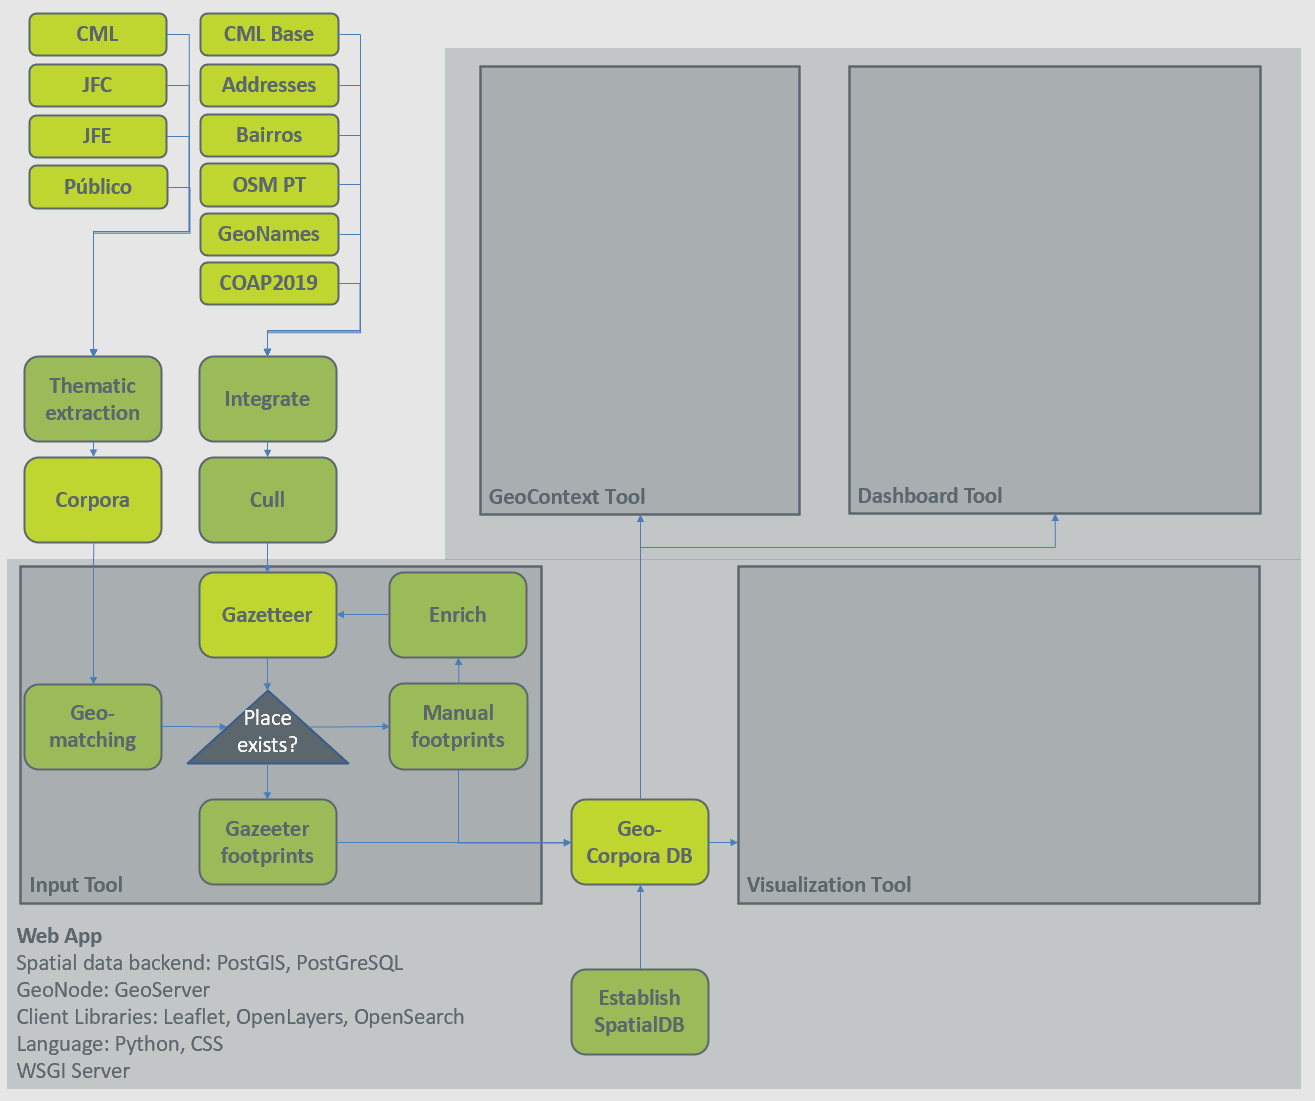
\includegraphics[width=.9\linewidth]{images/method_model.png}
	\caption{Preliminary methodology}
	\label{fig:method_model}
\end{figure}

\subsection{Preprocessing}
Load all gazetteer data into QGIS.
Establish georeference (note in data breakdown), transform as necessary
Manually code all article data. Using multiple sources to ensure continuity across local data sources.

\subsection{Initialization of development environment}
Selection and integration of resources and tools:
\begin{itemize}
	\item Database: PostgreSQL
\end{itemize}
Establish geodatabase structure, accommodating multiple language options, load gazetteer(s) and relevant administrative boundary data
Develop and test Input tool: wordpress plugin?
Develop and test search tool
Develop and test Context tool
Translate web app content to portuguese and load translations
Migrate site to the server
Test system
Compare results against mined location results
Document results

Future development: dashboard tool

\subsection{Tool design}
-{\color{red}Define design requirements and views to achieve them\cite{Zhang2019}}\\

\subsection{Testing}
- {\color{red}Test in different browsers for feature functionality.\cite{Shneiderman2020}}\\

\subsection{Validation}
1. GDELT: compare Lisbon Oct 2020 to results
2. Automatic extraction over sample corpora to compare results {\color{red} leverage Rivera2020 study}
- spaCy
-{\color{orange}``Large scale infomration extraction tasks''\cite{spaCy2020}}\\
-{\color{orange} Free online classes to learn\cite{spaCy2020}}\\
-{\color{purple}Utilize NER to extract exact and complete places.  As a baseline comparison to the input tool? Used together? Feed through the system with a “check point” (verify the identified place before input)?\cite{Gupta2020}}\\
-{\color{red}Use local datasets (Público, CML, Freguesia) from 1 month of each to build and test a backoffice plugin for defining localization of news articles. Ask MAGG or similar to apply the plug in for upcoming articles for a 1 month period and test against the same dataset with NewsStand. Is it richer/more accurate? Is the journalist satisfied with the result? Is the reader? Load the same local base gazetteer (OSM Portugal and Global)\cite{Lieberman2010}}\\
-{\color{red}Use method for extraction on input articles to extract and geolocate place for input comparison to automated methods?? Python and Restful API}\\
